\begin{table}[h!]
	\caption{The LogisticRegression parameters}
	\begin{tabular}{ | l | l | p{7cm} |}
		\hline
		\textbf{Parameter} & \textbf{Default} & \textbf{Description}\\
		\hline
		$C$ & 1.0 & Inverse of regularization strength; must be a positive float. Smaller values specify stronger regularization.\\
		\hline
		$penalty$ & l2 & ‘l1’ or ‘l2’. Used to specify the norm used in the penalization.\\
		\hline
		$class\_weights$ & None & Over-/undersamples the samples of each class according to the given weights. If not given, all classes are supposed to have weight one. The ‘auto’ mode selects weights inversely proportional to class frequencies in the training set.\\
		\hline
	\end{tabular}
	\label{table:LRdefaults}
\end{table}
The following set of hyper-parameter values was used:
\begin{itemize}
	\item C: 10\^-4:4
	\item penalty: ['l2', 'l1']
	\item class\_weights': [None, 'auto']
\end{itemize}
\subsubsection{Results}
\begin{table}[h!]
	\centering
	\caption{Grid search output}
	\begin{tabular}{ | l | c | c | c | c |}
		\hline
		$\bf{params_n}$ & \bf{C} &  \bf{penaly} & \bf{class\_weights} & \bf{log\_loss} \\ \hline
		$params_1$ & 0.2682 & 'l2' & 'auto' & 0.7952 \\ \hline
		$params_2$ & 0.2682 & 'l1' & 'auto' & 0.8175 \\ \hline
		$params_3$ & 0.0193 & 'l2' & None & 0.8245\\ \hline
		$params_4$ & 0.0719 & 'l2' & 'auto' & 0.8500 \\ \hline
		$params_5$ & 0.2682 & 'l2' & None & 0.8566 \\ \hline
	\end{tabular}
	\label{table:LR_gs}
\end{table}
\vspace{2mm}
\begin{figure}[h!]
	\centering
	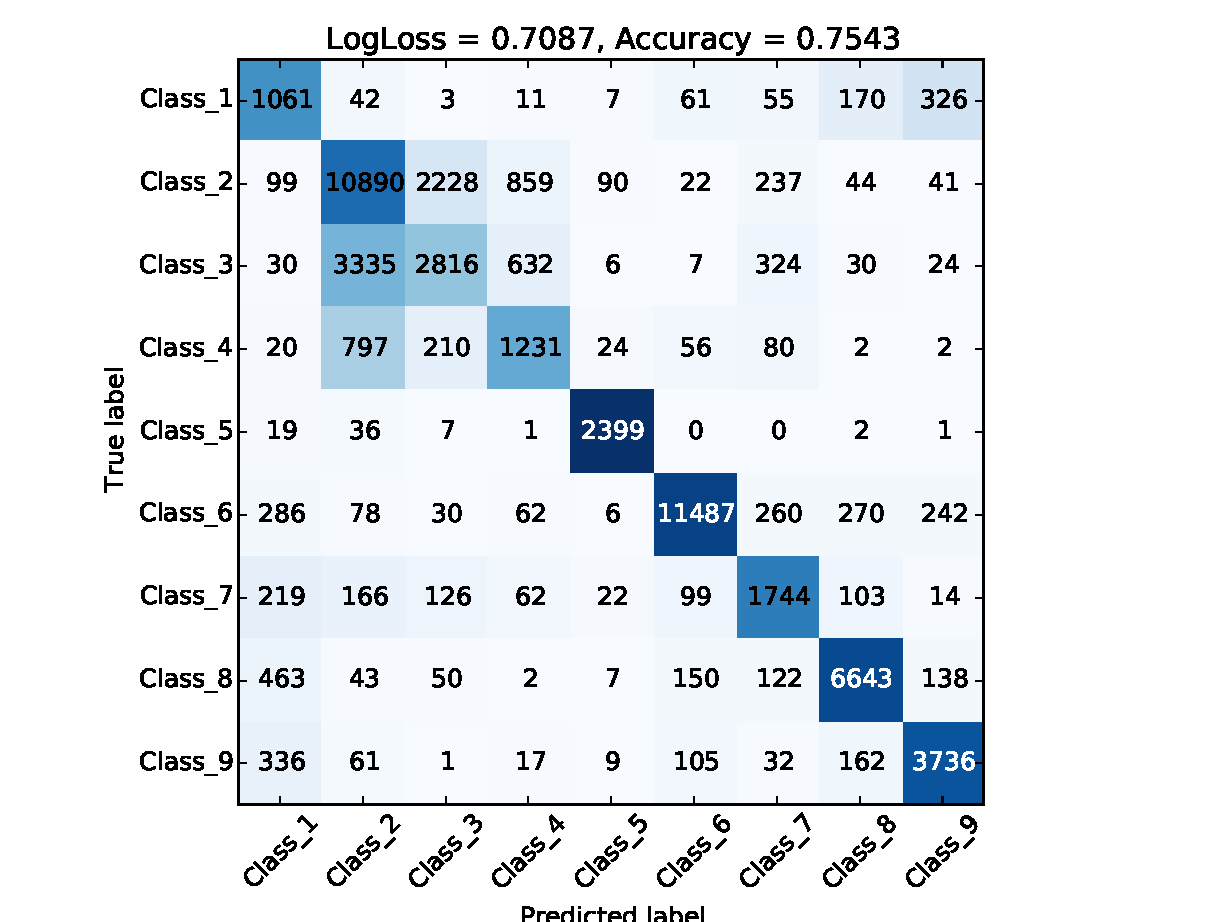
\includegraphics[width=0.7\textwidth]{LRcm_train}
	\caption{Logistic regression confusion matrix using training dataset}
	\label{fig:LRcm_train}
\end{figure}
\begin{figure}[h!]
	\centering
	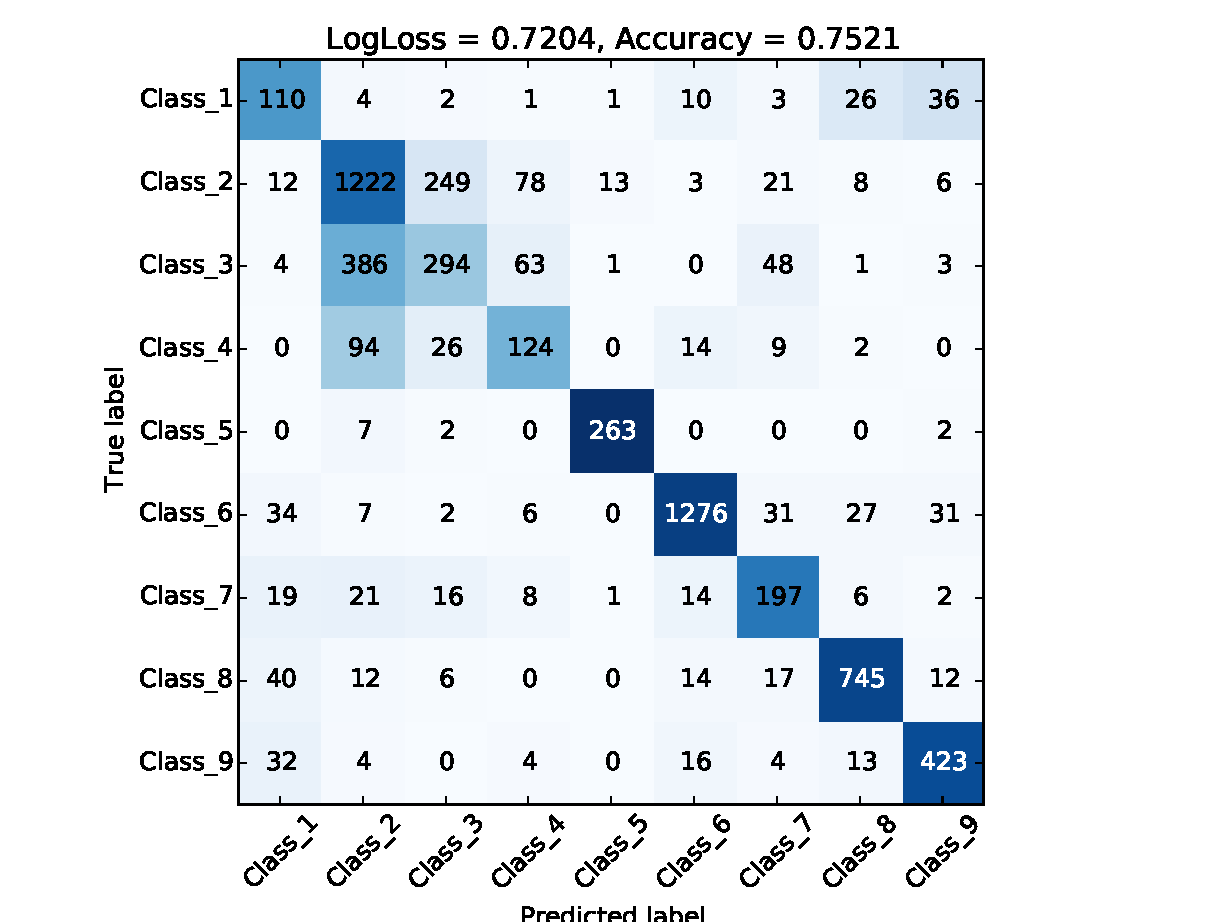
\includegraphics[width=0.7\textwidth]{LRcm_test}
	\caption{Logistic regression confusion matrix using testing dataset}
	\label{fig:LRcm_test}
\end{figure}
Performance using training and testing set is similar, but still not good enough. A lot of misclassifications are made among classes, specially between class 2 and 3.